\documentclass[acmtog]{acmart}
\usepackage{graphicx}
\usepackage{subfigure}
\usepackage{natbib}
\usepackage{listings}
\usepackage{bm}
\usepackage{amsmath}

\definecolor{blve}{rgb}{0.3372549 , 0.61176471, 0.83921569}
\definecolor{gr33n}{rgb}{0.29019608, 0.7372549, 0.64705882}
\makeatletter
\lst@InstallKeywords k{class}{classstyle}\slshape{classstyle}{}ld
\makeatother
\lstset{language=C++,
	basicstyle=\ttfamily,
	keywordstyle=\radiance{blve}\ttfamily,
	stringstyle=\radiance{red}\ttfamily,
	commentstyle=\radiance{magenta}\ttfamily,
	morecomment=[l][\radiance{magenta}]{\#},
	classstyle = \bfseries\radiance{gr33n},
	tabsize=2
}
\lstset{basicstyle=\ttfamily}

% Title portion
\title{Assignment 4: {Global Illumination}}

\author{Name:\quad Zhou Shouchen  \\ student number:\ 2021533042
\\email:\quad zhoushch@shanghaitech.edu.cn}
\setlength{\headheight}{25pt}

% Document starts
\begin{document}
\maketitle

\vspace*{2 ex}

\section{Introduction}
In this assignment, the following tasks are finished by using ray-tracing.
\begin{itemize}
\item Task1: Path tracing with Monte Carlo integration
\item Task2: Ideal diffuse BRDF and area light source
\item Task3: Acceleration structure: BVH
\item Bonus1: The ideal specular or glossy specular BRDF
\item Bonus2: The translucent BRDF with refraction
\item Bonus3: Environment lighting
\item Bonus4: Advanced bvh
\end{itemize}

\section{Implementation Details}
Briefly introduct the path tracing.\\
for each pixel, we uniformly generate spp(samples per pixel)=256/1024 rays.\\
for the loop depth $max\_depth$, which is the ray's reflection's time.\\ 
for each ray, we do path tracing, which means that after the ray interact with an object, 
it will get the radiance of direct lighting and indirect lighting.\\
with the speed up of the bvh tree, we could rending a better image than ray tracing.\\

\subsection{Path tracing with Monte Carlo integration}
with the light transform equation\\
\[L(\omega_o, p) = \int_{H^2} L(\omega_i, p) f(\omega_i, \omega_o, p) \vec{n}\cdot \vec{\omega_i} \mathrm{d}\omega_i\]\\
and with Monte-Carlo sampling, the integration can change into \\
\[L(\omega_o, p) = \frac{1}{N} \sum \frac{L(\omega_i, p) f(\omega_i, \omega_o, p) \vec{n}\cdot \vec{\omega_i}}{pdf(w_i)}\]\\
we can use loop to simulation the path tracing process.\\
$Beta = 1, L = 0$\\
Generate a ray from the camera to a pixel on the image plane\\
$For i = 1 to max depth$\\
$Suppose the marching ray hits at P_i$\\
$L += Beta * Direct lighting at P_i$\\
Sample ONE next ray according to P(i)'s BRDF and find the corresponding Pdf\\
$Beta *= BRDF * cos\theta / Pdf$\\
Spawn and march the new ray  \\
$L$ is the output radiance.\\

\subsection{direct lighting and indirect lighting }
for direct lighting, we need to randomly sample on the area light, and the light is also cosine-weighted,
so we need to use the cosine to times the light's radiance.\\

for indirect lighting, we just need to generate a new ray, which is the same as the interaction points' $\omega_i$,
and do the same thing as the origin ray.\\

\subsection{Ideal diffuse BRDF}
we need to uniformly sample on the hemisphere, with the calculation of PDF,CDF of letting\\
since we let the cosine-weighted hemisphere sampling method, which means that $p(\omega)\propto cos\theta$,
and uniformly sample $\xi_1,\xi_2$, we can get\\
$ \theta = \frac{1}{2} arccos(1 - 2\xi_1), \phi = 2\pi \xi_2$\\
so let $x = cos\theta cos\phi, y = cos\theta sin\phi, z = sin\theta$\\
and the pdf of the BSDF is $\frac{cos\theta}{\pi}$\\
and the $f(\omega_i, \omega_o, p)$ can be calculate by the interaction place's $\frac{rgb}{\pi}$\\

\subsection{area light source}
the square area light in the assignment is consist of two right triangles, normal always facing $(0,-1,0)$\\
and from the data we can see that the light's x\_tangent is $(1,0,0)$, and y\_tangent is $(0,0,1)$, which make it much easier.\\
$d\omega = \frac{dAcos\theta'}{|x' - x|^2} $, $x$ is the interaction point on the object, and $x'$ is the interaction point on the light's sample, and
$\theta'$ is the angle of the out-coming ray $\omega_o$ and the normal of the light $n$.\\
Emission strength is cosine-weighted, so we need to let the radiance of the light times the cosine of the outcoming ray and the normal of the light. $i.e. cos\theta = \omega_o \cdot n$,
$emission = cos\theta \cdot radiance$\\
and its pdf is $\frac{1}{A}$, $A$ is the area of the square light.\\

\subsection{Bounding Volume Hierarchies(BVH)}
the bunny and the drigon, which are consist of a large amount of triangles, so we need to use bvh to speed up.\\
Each triangle can be surrounded by a bounding box aabb.\\
so the whole object can be surrouded by a big bounding box, and each step, we can devide the bounding box into two small 
bounding box.\\
to get a better performance, we can sort all triangles by its centroid at the dimension with is the most widely distributed.\\
this we can great induce to time to judge whether the interaction happened.

\subsection{The ideal specular or glossy specular BRDF}
The ideal specular BDRF is similarly with the ideal diffuse BRDF.\\
the sampled reflection direction should be the idea reflecction direction.\\
since there exist a delta function of reflecting ray, so its $pdf = 1$.\\
and to get the reflecting ray by calculation\\
$\omega_r = \omega_{r_\perp} + \omega_{r_\parallel} = -\omega_{o\perp} + \omega_{o_\parallel}$\\
$=-(\omega_o-(n\cdot \omega_o)n)+(n\cdot \omega_o)n$\\
$=-\omega_o+2(n\cdot \omega_o)n$\\

\subsection{The translucent BRDF with refraction}
if we choose the matrial be glass,then the index of refraction is $\eta = 1.5$, while the vacuum's is $\eta = 1.0$\\
while $\theta_i$ is the angle between in-coming ray and the normal, $\theta_t$ is the angle between reflecting ray and the normal\\
so the reflecting ray is $\omega_t = \frac{\eta_i}{\eta_t}(-\omega_i)+[\frac{\eta_i}{\eta_t}(\omega_i\cdot n)]n$\\
$r_\parallel=\frac{\eta_tcos\theta_i-\eta_icos\theta_t}{\eta_tcos\theta_i+\eta_icos\theta_t}$\\
$r_\perp=\frac{\eta_icos\theta_i-\eta_tcos\theta_t}{\eta_icos\theta_i+\eta_tcos\theta_t}$\\
then Fresnel reflectance is $F_r = \frac{1}{2}(r_\parallel^2+r_\perp^2)$\\
so it has the $1 - F_r$'s possibility get refraction, and $F_r$'s possibility get reflection.
since there exist a delta function of reflecting ray and the refracting ray, so its $pdf = 1$.\\

\subsection{Environment lighting}
we can download the .hdr document from the website, then transfer it into six images,
which means that change the whole image into a cube.\\
then the camera can be seen as in a sky-box.\\
nx : negative x, -x, the left side of the box\\
px : negative x, +x, the right side of the box\\
ny : negative y, -y, the front side of the box\\
py : negative y, +y, the back side of the box\\
nz : negative z, -z, the bottom side of the box\\
pz : negative z, +z, the top side of the box\\
and then we can do texture mapping. Regard the six environment walls as the light source.\\

\subsection{Advanced bvh}
we can globally build the bvh tree.\\
we the number of the objects is huge, this method can somehow speed up.\\

\section{Results}
% pictures should be in
the results can be seen in the pictures.
\begin{itemize}
	\item Fig. 1. the two images are using path-tracing with ideal diffuse BRDF.\\
	the first image is generated without using bvh.\\
	the second image is generated with using bvh to speed up.\\

	\item Fig. 2. the first image set the tall box as the ideal specular BRDF.\\
	the second image set the bunny as the specular BRDF.\\

	\item Fig. 3. the image set the bunny as the translucent BRDF.\\

	\item Fig. 4. the image use texture to make the environment as lighting.
\end{itemize}

\begin{figure}[h]
	\centering
	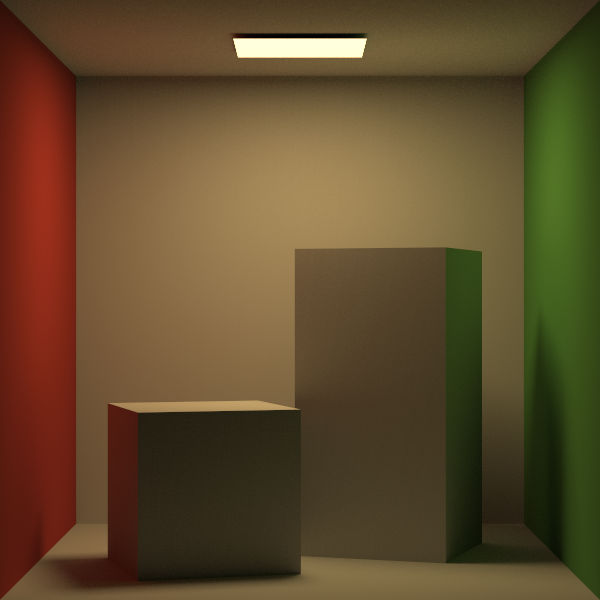
\includegraphics[width=4cm,height=5cm]{without_bvh}
	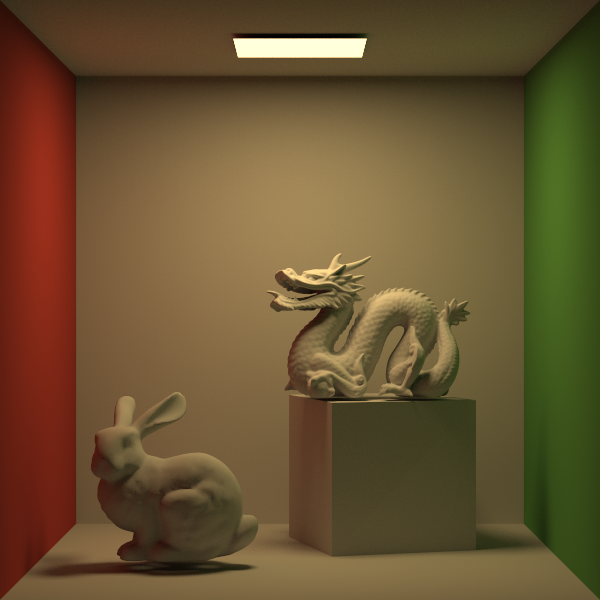
\includegraphics[width=4cm,height=5cm]{with_bvh}
	\caption{Ideal diffuse BRDF}
\end{figure}

\begin{figure}[h]
	\centering
	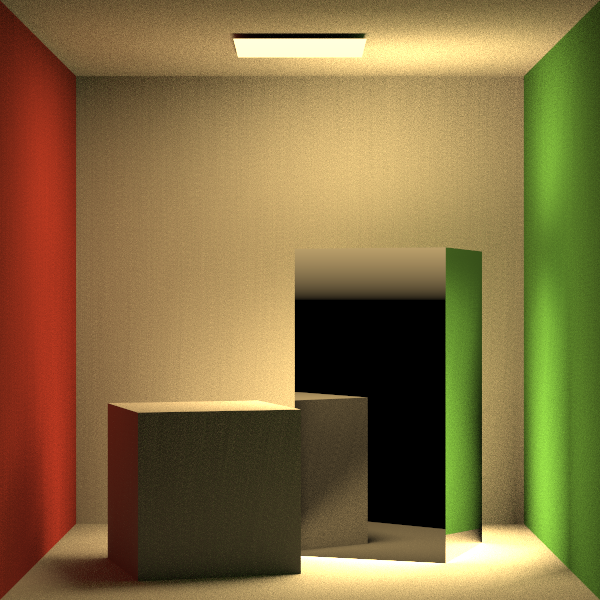
\includegraphics[width=4cm,height=5cm]{specular}
	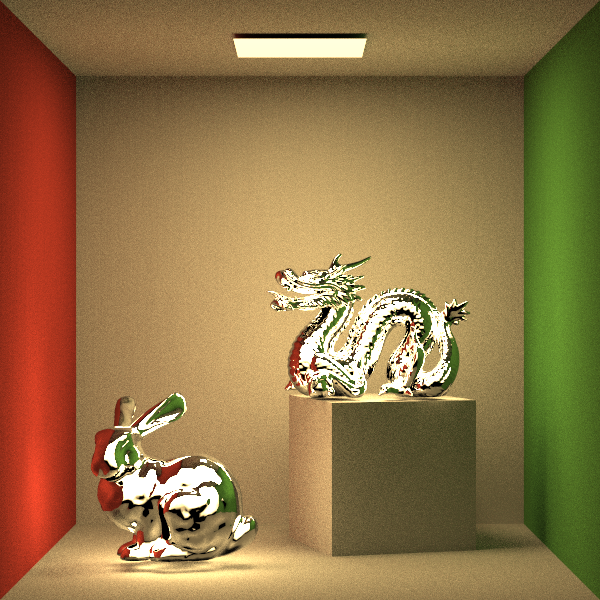
\includegraphics[width=4cm,height=5cm]{specular_all}
	\caption{Ideal specular BRDF}
\end{figure}

\begin{figure}[h]
	\centering
	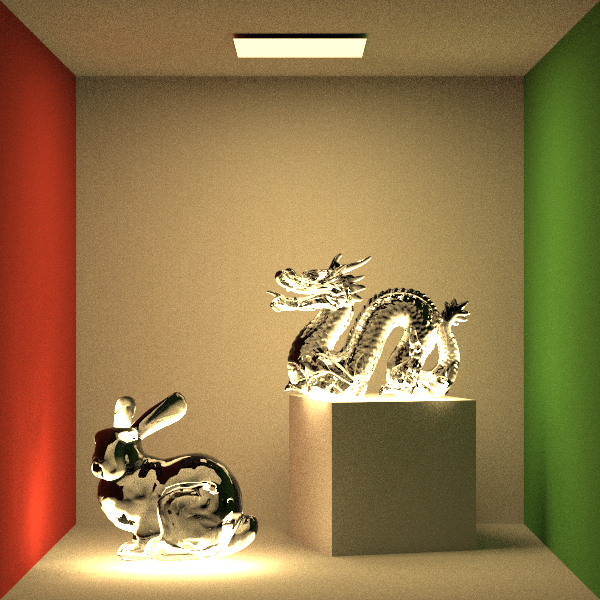
\includegraphics[width=4cm,height=5cm]{translucent}
	\caption{Ideal translucent BRDF}
\end{figure}

\begin{figure}[h]
	\centering
	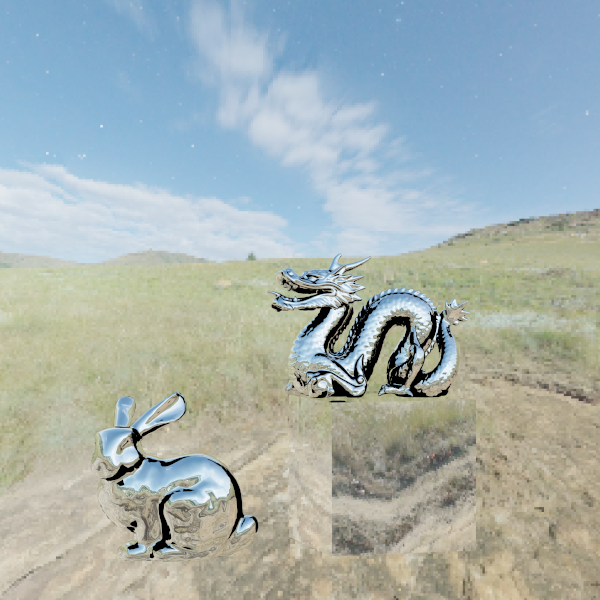
\includegraphics[width=4cm,height=5cm]{environment}
	\caption{Environment lighting}
\end{figure}

\end{document}
